%!TEX root=document.tex

\section{Experimental Evaluation}

We evaluated the performance of \SeeDB\ on a variety of datasets with different
sizes and number of attributes. We now discuss in detail the effect of
each of our optimization strategies and develop an analytical model that lets us
pick the optimial settings of \SeeDB\ parameters.

\subsection{Experimental Setup}

\begin{table}[htb]
  \centering \scriptsize
  \begin{tabular}{|c|c|c|c|c|c|c|} \hline
  Type & Dataset & Num  & Num  & Num  & Size (GB) &
  Num \\
  & Name & Rows & Dimensions &  Measures & & Views \\ \hline 
   & $Small_1$ & 1M & 5 & 2 &  0.1 & \\ 
  Small & $Small_2$ & 10M & 5 & 2 &  1 & 10\\ 
   & $Small_3$ & 100M & 5 & 2 &  10 & \\ \hline
   & $Med_1$ & 1M & 50 & 5 &  0.4 & \\
  Medium & $Med_2$ & 10M & 50 & 5 &  4 & 250\\ 
   & $Med_3$ & 100M & 50 & 5 &  40 & \\ \hline
   & $Large_1$ & 1M & 100 & 10 &  1 & \\
  Large & $Large_2$ & 10M & 100 & 10 &  10 & 1000\\
   & $Large_3$ & 100M & 100 & 10 &  100 & \\ \hline
  \end{tabular}
  \caption{Datasets used for testing}
  \label{tab:datasets} 
\end{table}

Table \ref{tab:datasets} lists the datasets on which we evaluated the
performance of \SeeDB. These datasets are synthetically generated and their size
varies from 100 MB to 100 GB and number of attributes ranges from 5 - 100 dimension attributes and 2 -
 10 measure attributes. The relative cardinality of dimension and measure attributes
was chosen to model real-world datasets which usually have a large number of
dimension attributes but few measure attributes. To accurately estimate the
effect of specific optimizations, for each dataset, we also created a
supplemental dataset with the same specifications except that each attribute had
the same number of distinct values (100).

For each dataset, we used \SeeDB\ to find the top 20 views of the input query.
Any run that took more than 1 hour was terminated. All experiments were repeated
three times and the results were averaged.
We ran experiments using Postgres as the backend database for \SeeDB\ and a single
machine with 32 Intel Xeon E7 processors with hyperthreading enabled and 256 GB
RAM.

\subsection{Effect of Optimizations}
\label{sec:experiments}
We now present experimental characterization of the optimization
strategies described in \ref{subsec:seedb_backend}. Our goal is to understand
the effect of each strategy on \SeeDB\ performance in order to build an
analytical model and predict the optimal set of parameters for \SeeDB.

\subsubsection{Basic Framework}
We first examined the baseline performance of \SeeDB\ without any optimizations.
For each possible view, we executed the target and comparison view queries
separately and sequentially, and then picked the top views. This corresponds to
the basic framework described in Section \ref{sec:basic_framework}. The number
of queries executed for each dataset was twice the number of views shown in
Table \ref{tab:datasets}. Figure \ref{fig:baseline_performance} shows the baseline
performance for Small, Medium and Large datasets of size 1M. We observe that
execution time increases super-linearly as the size of the dataset (number of dimension and
measure attributes) increases. Moreover, as mentioned before, even for the
Medium sized dataset (1M rows, 5 measure and 50 dimension attributes), \SeeDB\
execution takes 700s, a latency that is unacceptable for interactive queries.

\begin{figure}[h]
  \centering
    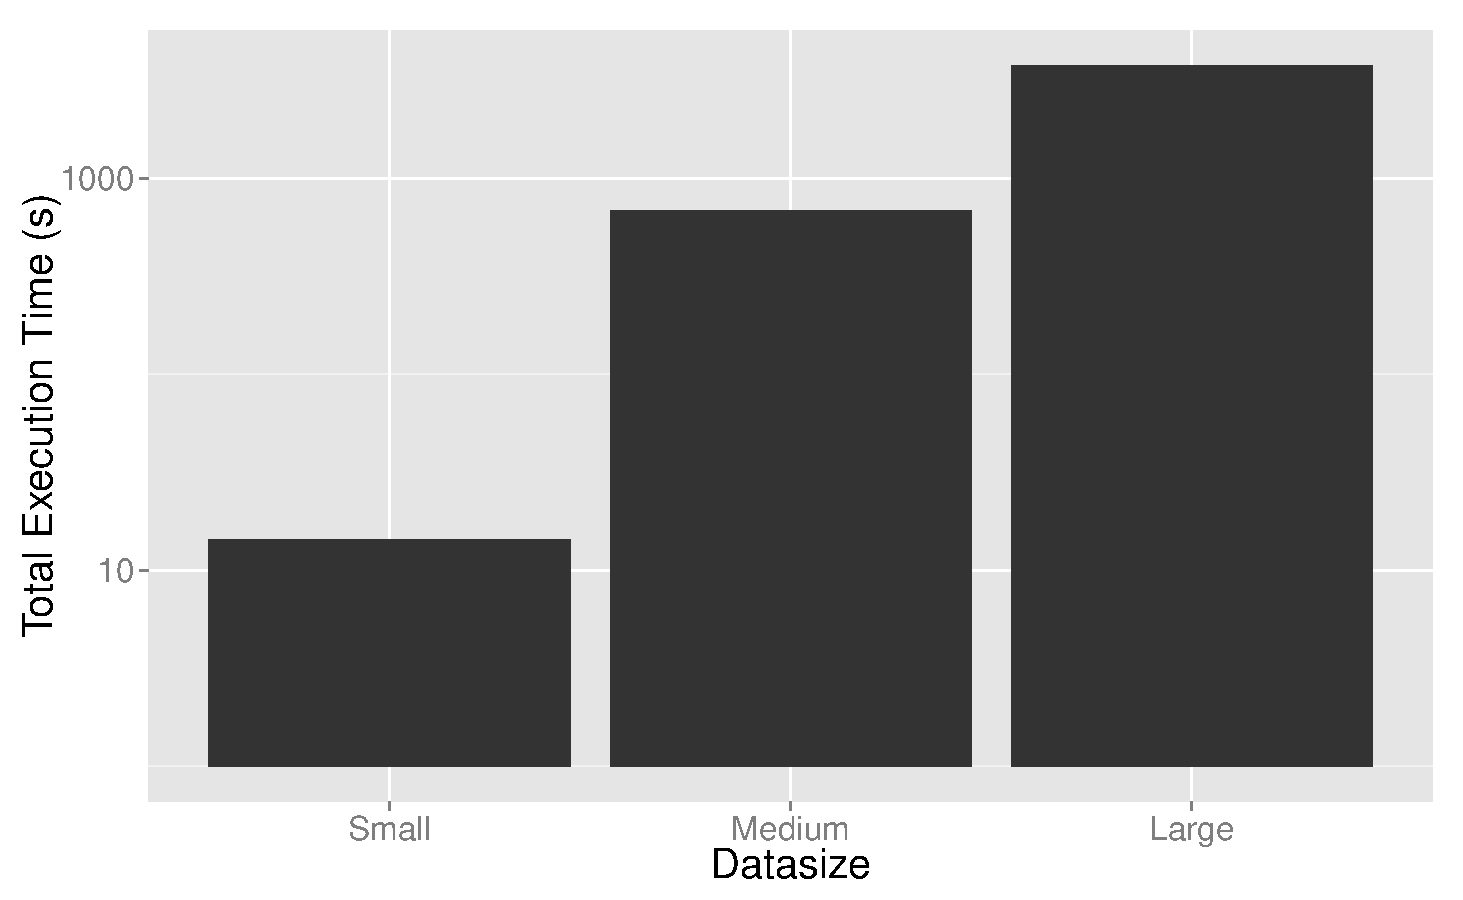
\includegraphics[width=6cm]{Images/baseline_performance.pdf}
    \caption{Baseline Performance} 
      \label{fig:baseline_performance}
\end{figure}

\subsection{Combine target and comparison view query}
Next, we study the effect of combining target and comparison view queries as
described in Section \ref{subsec:target_comparison_view}. The goal of this
optimization is to execute both queries in a single scan of the table.
Therefore, the total number of queries executed is equal to the number of
views possible for a given dataset. This optimization offers an average speed up
of 1.7x across a range of selectivities for the input query.

\subsubsection{Combine Multiple Aggregates}
\SeeDB\ uses the parameter $n_{agg}$ to denote the number of aggregates that may
be included in the same view query. Therefore, given a set of view queries with
the same group-by attribute, view queries are combined so that each query has up
to $n_{agg}$ aggregates. We varied $n_{agg} \in {2, 3, 5, 10}$ for each dataset
(Note that the Small and Medium dataset have only 2 and 5 measure attributes
respectively).
Figure \ref{fig:mult_agg} shows the performance gains achieved for the 1M row
datasets. We see that for a given dataset, increasing $n_{agg}$, i.e. computing
more aggregates in the same query, gives an almost linear speedup. We also
notice that this optimization is slightly more effective for larger datasets.

\begin{figure}[h]

  \centering
    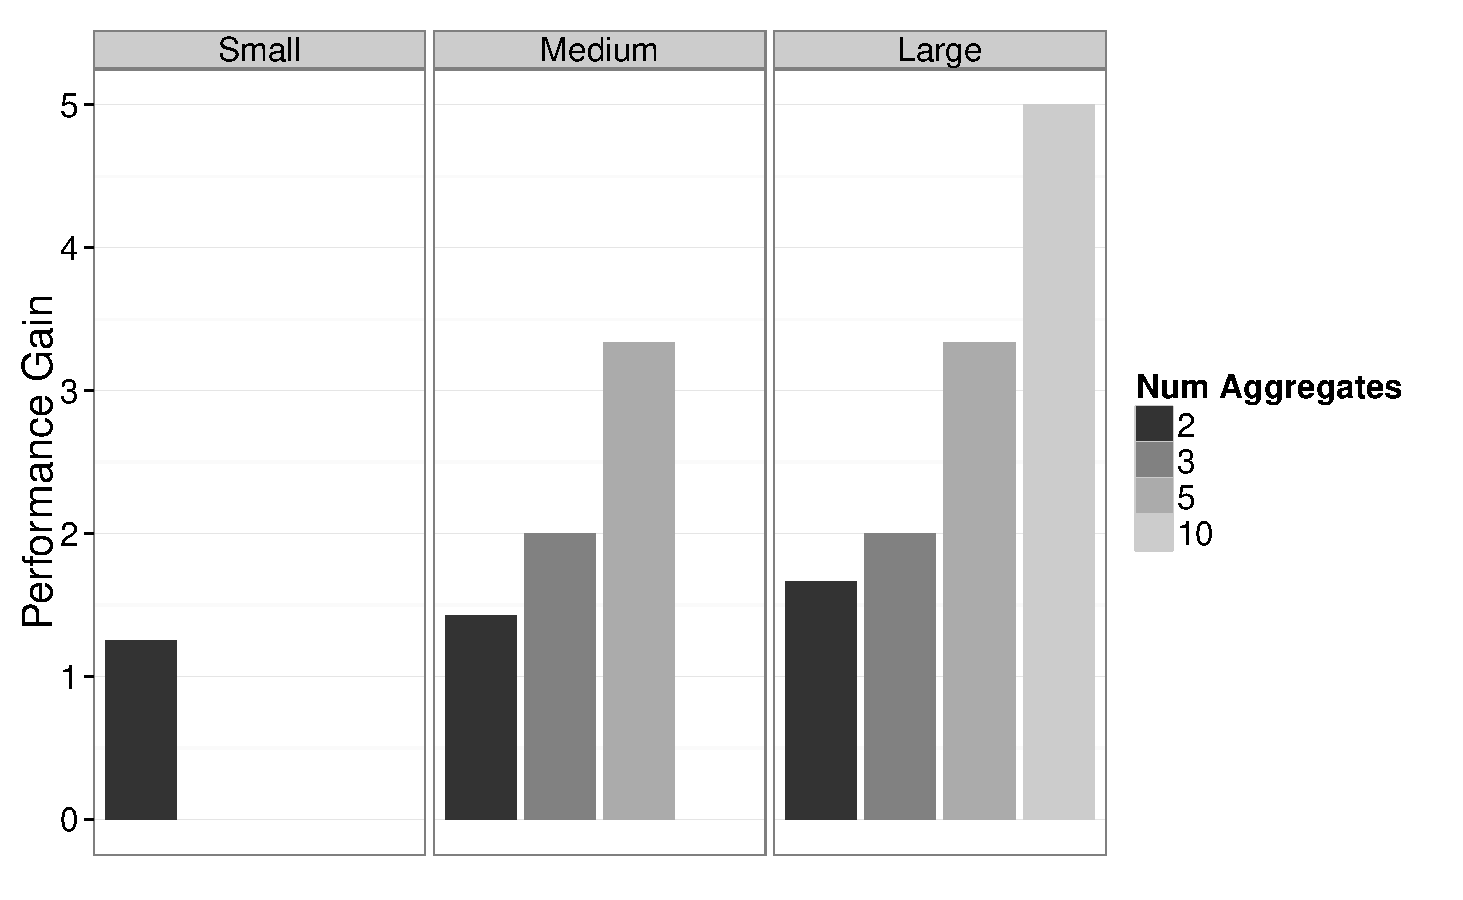
\includegraphics[width=6cm]{Images/mult_agg.pdf}
    \caption{Effect of Multiple Aggregate Optimization} 
      \label{fig:mult_agg}
\end{figure}

\subsubsection {Parallel Query Execution}
As discussed in Section \ref{subsec:parallel_exec}, executing view queries in
parallel can provide significant performance gains; however, a high degree of
parallelism can lead to a performance drop off for several reasons. Potential
reasons include disk contention, RAM usage, lock contention, context switches
and cache line contention
\cite{Postgres_wiki}.
Identifying the right amount of parallelism requires tuning for the particular
workload. The \SeeDB\ workload consists of multiple parallel queries performing
full sequential scans of a given table. To evaluate the
effect of parallelism, we varied the number of queries that can be executed in
parallel and measured its effect on the average time to execute a query as well
as the total execution time. Since our backend DBMS is Postgres, parallel query
execution is implemented by opening multiple connections and running queries
sequentially on each connection.

Figure \ref{fig:parallelism} shows the effect of parallelism on the average
execution time per view (Medium dataset, 1M rows). Note the log scale on the
y-axis.
We observe that query execution time stays flat between 1 - 10 connections, suddenly increases between
10 - 20 connections, and then increases linearly for more than 20 connections.
This suggests that the benefits of parallel execution are outweighed by
contention beyond 20 connections. Figure \ref{fig:parallelism_total} shows the
total time (as opposed to per view execution time) taken by \SeeDB\ for varying
levels of parallelism. We observe that the minima occurs in the range between 10
- 20 parallel queries and the execution times flatten out after 40 parallel
queries.
This trend is the effect of two opposing factors: (A) increased parallelism
increases contention, and therefore increases per query execution time, and (B)
parallelism decreases the number of batches of queries that must be executed,
thus reducing overall time.
We will take these two opposing forces into account when we develop an
analytical model for \SeeDB\ execution time in Section \ref{sec:model}.

\begin{figure}[h]

  \centering 
    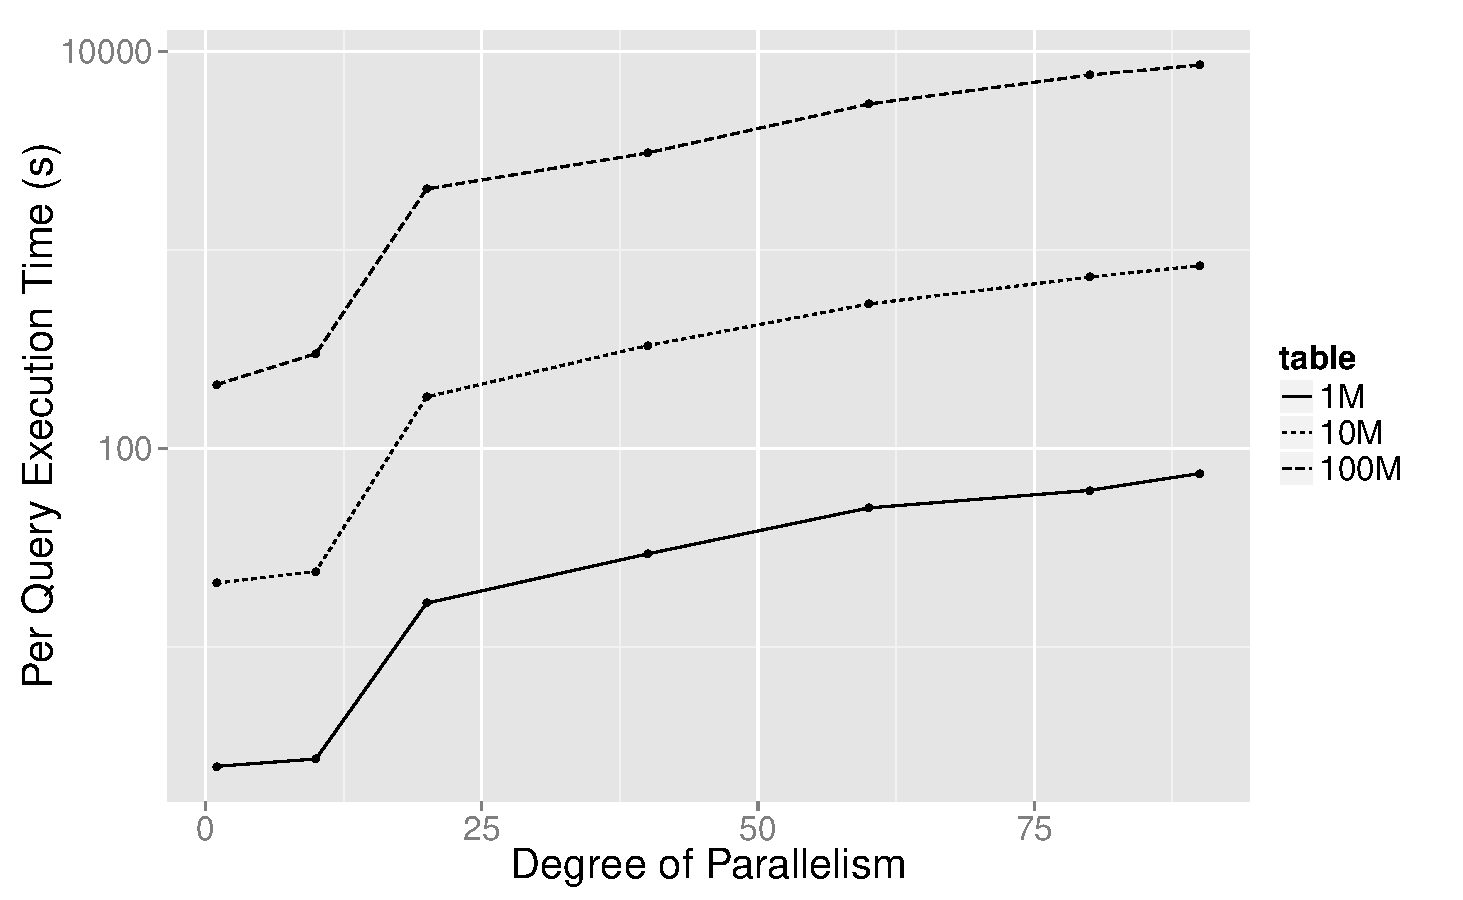
\includegraphics[width=6cm]{Images/parallelism.pdf}
      \caption{Effect of Parallelism on Per View Execution Time} 
        \label{fig:parallelism}
\end{figure}



\begin{figure}[h]


  \centering
    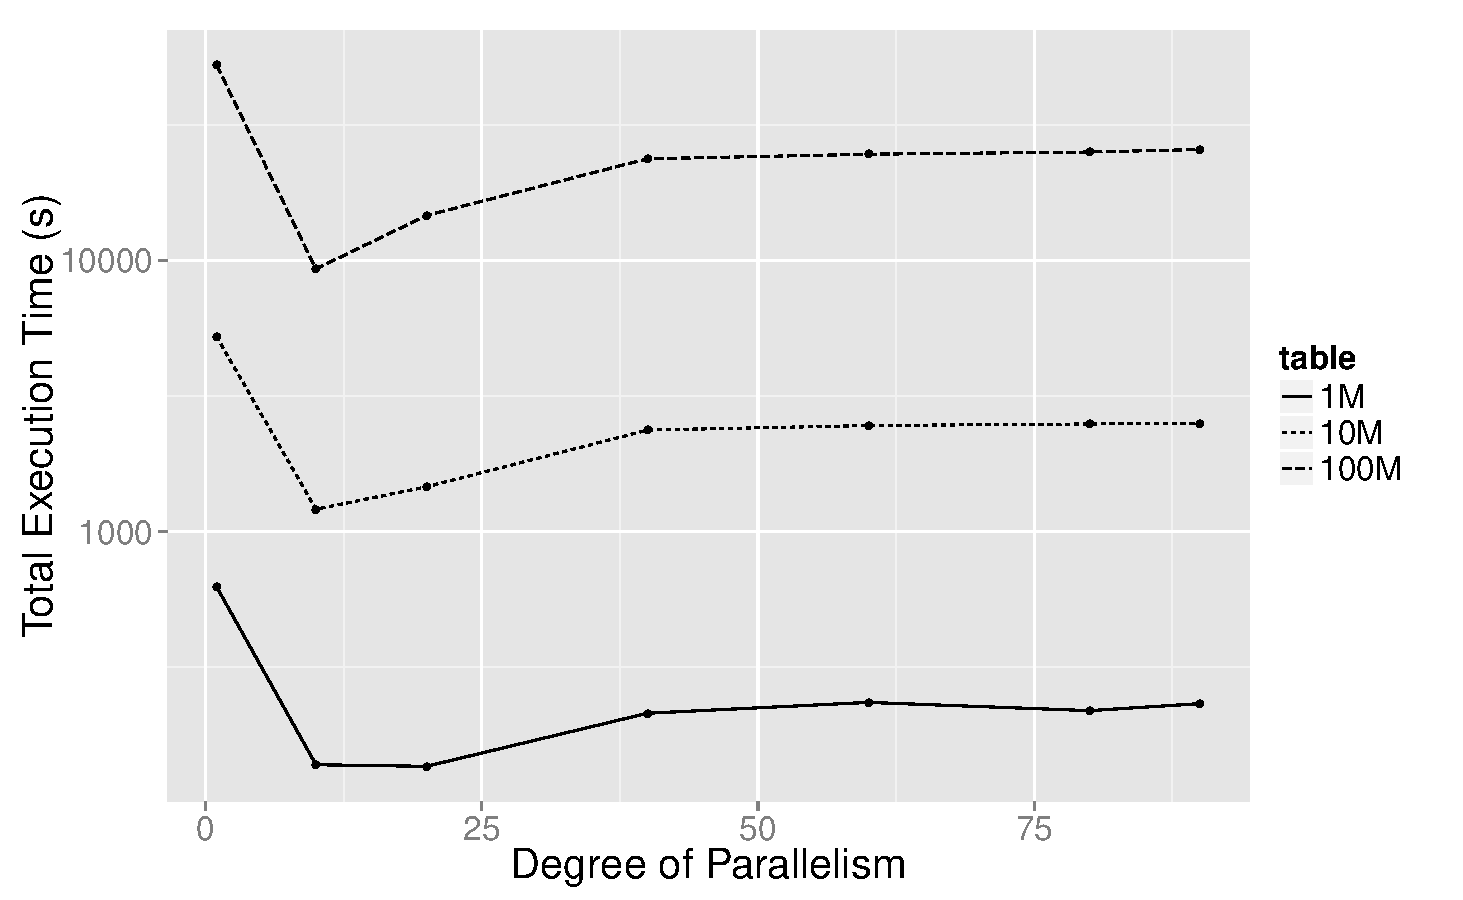
\includegraphics[width=6cm]{Images/parallelism2.pdf}
  \caption{Effect of Parallelism on Total Execution Time} 
    \label{fig:parallelism_total}
\end{figure}

\subsubsection {Combine Multiple Group-bys}
\label{subsec:mult_gb_expt}
Combining multiple attributes in a group-by clause can reduce the number of
views that must be explored individually.
However, the benefits of this optimization can be lost to high intermediate
result cost if the number of distinct groups is large. As mentioned before, we
divide this optimization into two phases:
(1) {\it Temp Table Creation} and (2) {\it Temp Table Querying}. In the first
phase, we run queries with grouping based on multiple attributes and store the
results in temporary tables. In the second phase, we run single
aggregate+group-by queries on the temp tables to obtain final results for views.
For instance, suppose that we want to compute the results for views ($a_1$, $m$,
$f$), ($a_2$, $m$, $f$) and ($a_3$, $m$, $f$). Instead of executing these views
individually, we combine these three views into a single view, (\{$a_1$, $a_2$,
$a_3$\}, $m$, $f$), which computes the aggregate for attribute $m$ using
function $f$ and groups by the attributes \{$a_1$, $a_2$, $a_3$\}. The results
of this query are stored in a temporary table which is then queried to get
results for the original views, ($a_1$, $m$, $f$), ($a_2$, $m$, $f$) and ($a_3$,
$m$, $f$).

\SeeDB\ uses the parameter $n_{GB}$ to denote the number of attributes in the
group-by clause. To evaluate the effect of combining group-bys, we ran \SeeDB\
by varying number of group-by attributes, i.e. the $n_{GB}$ parameter, between 1
and the number of dimensions $d$ in a given table. For each run, we measured the
amount of time taken to create the temporary tables, the time taken to query the
temporary tables and the total execution time. Figure
\ref{fig:avg_tt_creation} to \ref{fig:total_time} show the
results for the Medium dataset of size 1M tuples.

{\bf Temp Table Creation Phase}: Figure \ref{fig:avg_tt_creation} shows the
average time required to create temporary tables for $n_{GB}$=1\ldots50. There
are several points to note in this graph: (1) for $n_{GB}>=10$, the number of
connections does not have a significant impact of the temp table creation time.
We see this behavior because for $n_{GB}>=10$, the number of temp tables created
is $<=5$ and therefore a maximum of 5 connections is used irrespective of the
number of connections that are open.
We also note an upward trend in the total temp table creation time with
increasing $n_{GB}$ because the temporary tables gradually become larger in size
(the number of rows in the table is bounded by the number of rows in the input
table but an increase in $n_{GB}$ increases the columns present in the table).
We also observe that the ``sweet spot'' for temp table creation occurs between 1 -
2 group-bys. 

% Note that the time required for temp table creation is roughly
% proportional to the size of the temp tables. We leverage this fact when we
% develop the analytical model in the next section.

\begin{figure}[h]
  \centering
    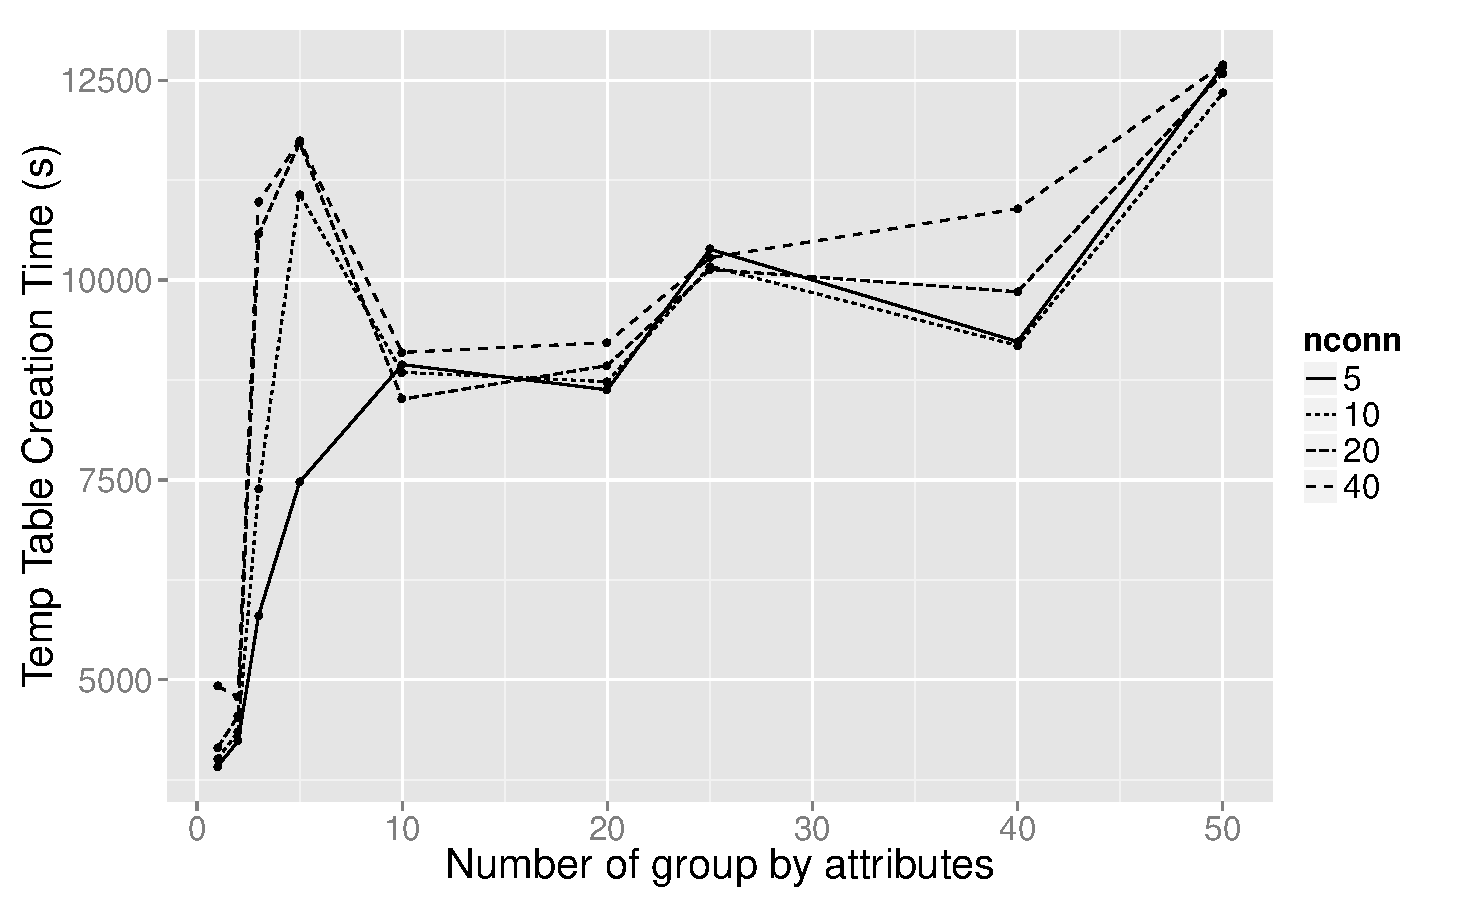
\includegraphics[width=6cm]{Images/mult_gb_tt_creation_single.pdf} 
  \caption{Average Temp Table Creation Time} 
    \label{fig:avg_tt_creation}
\end{figure}

\begin{figure}[h]
  \centering
    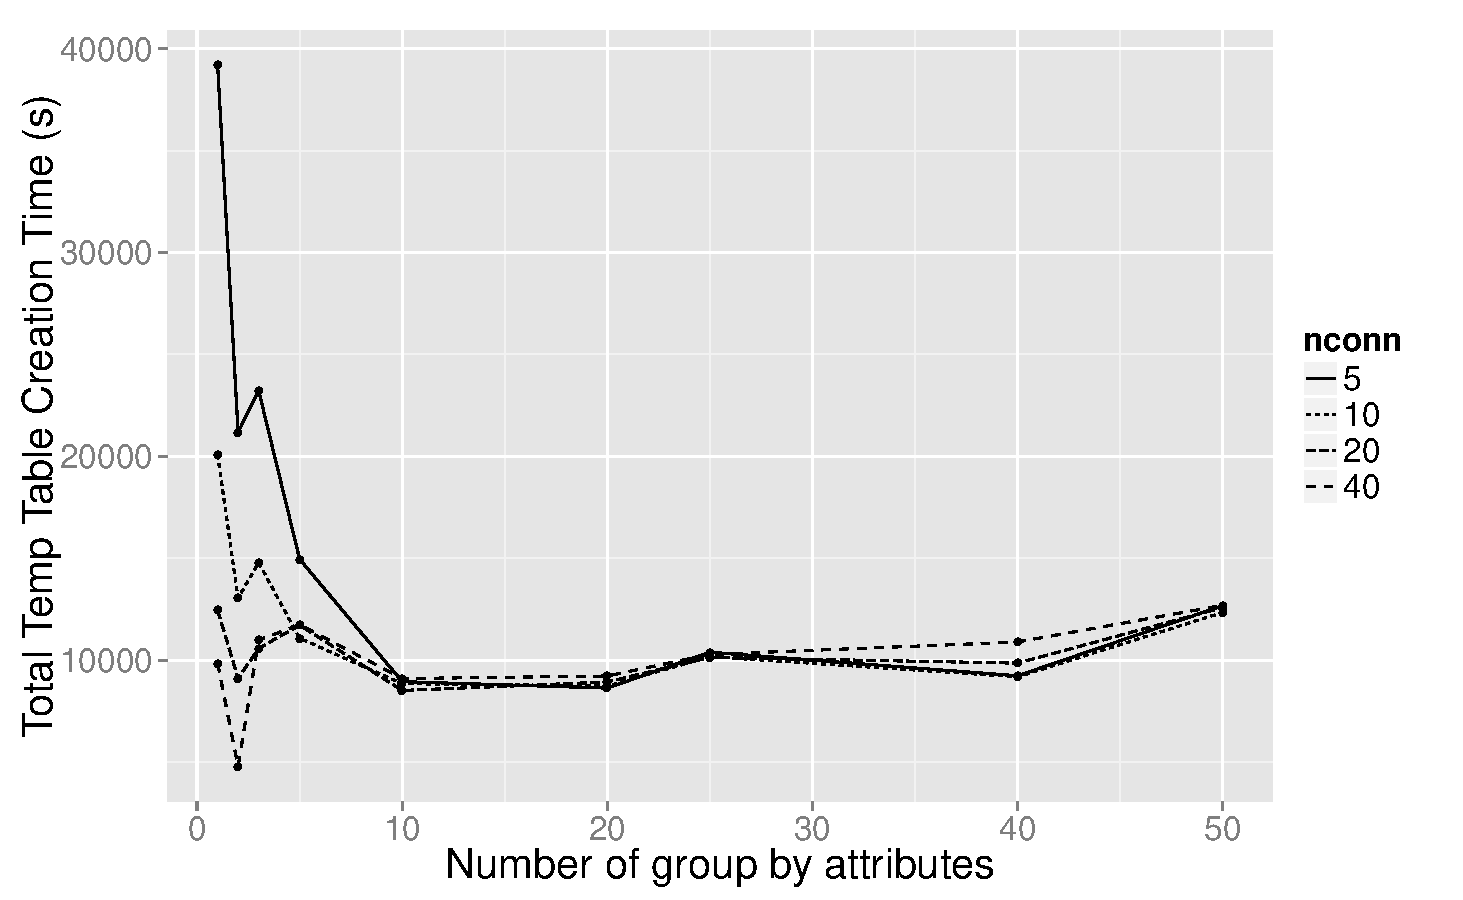
\includegraphics[width=6cm]{Images/mult_gb_tt_creation_total.pdf}
  \caption{Total Temp Table Creation Time} 
    \label{fig:total_tt_creation_time}
\end{figure}

Figure \ref{fig:total_tt_creation_time} shows the total time spent in creating
temporary tables in \SeeDB. As before, we see that the total time
flattens out after 10 group-bys; however, we observe a reordering of the the
trend lines with respect to number of connections. While the average time taken
to generate temp tables with 5 connections is the least, \SeeDB\ must run more
batches of queries to create the required number of temporary tables. We observe
that that 40 connections is optimal for minimizing the total temp table creation
time. As in the previous diagram, we observe a minima around $n_{GB}=2$.

{\bf Temp Table Query Phase}: Figures \ref{fig:avg_tt_query_time} and
\ref{fig:total_tt_query_time} respectively show the average time required to run
each view query on the temp tables and the total time to run all view queries.
Note that for the Medium dataset, there are 250 possible views and therefore 500
view queries that are to be run against the database.

In Figure \ref{fig:avg_tt_query_time}, we see clear trends in  the average time
taken to execute view queries on temp tables. Specifically: (1) The time taken
to query a temp table increases non-linearly with the number of queries
executing in parallel. We see that the trend lines are ordered by number of
connections and the loss of performance grows with number of connections. (2) As
before, we observe a slight increase in the execution time as the size of temp
tables increases. This is not surprising since the query executor must scan and
process more data. (3) Finally, we observe a minima at $n_{GB}=2$, similar the to
two graphs above.


\begin{figure}[h]
  \centering
    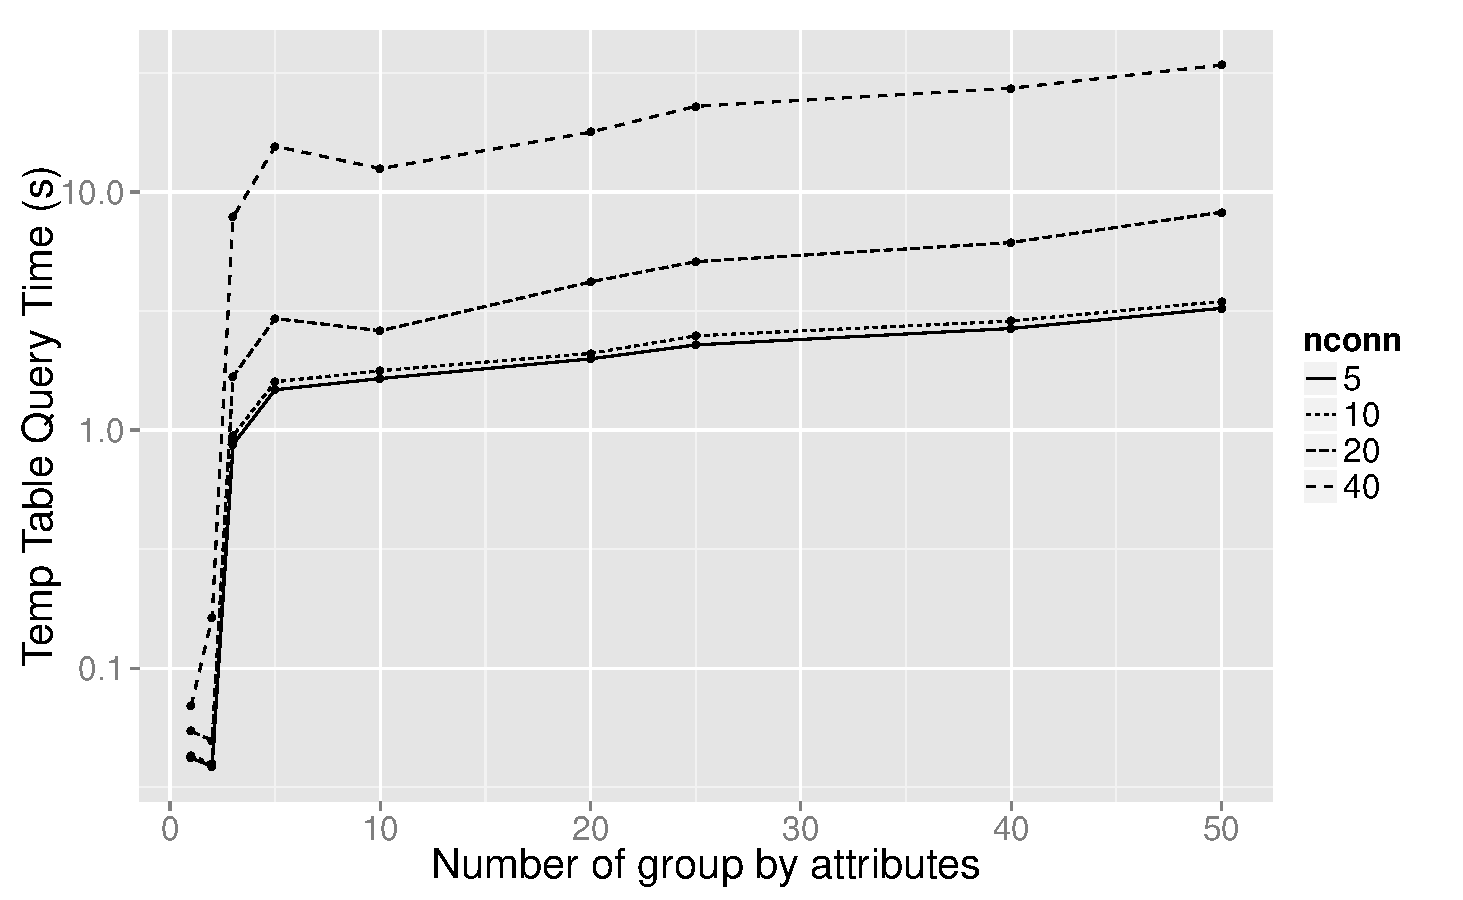
\includegraphics[width=6cm]{Images/mult_gb_tt_query_single.pdf}
  \caption{Average Temp Table Query Time}
  \label{fig:avg_tt_query_time}
\end{figure}

\begin{figure}[h]
  \centering
    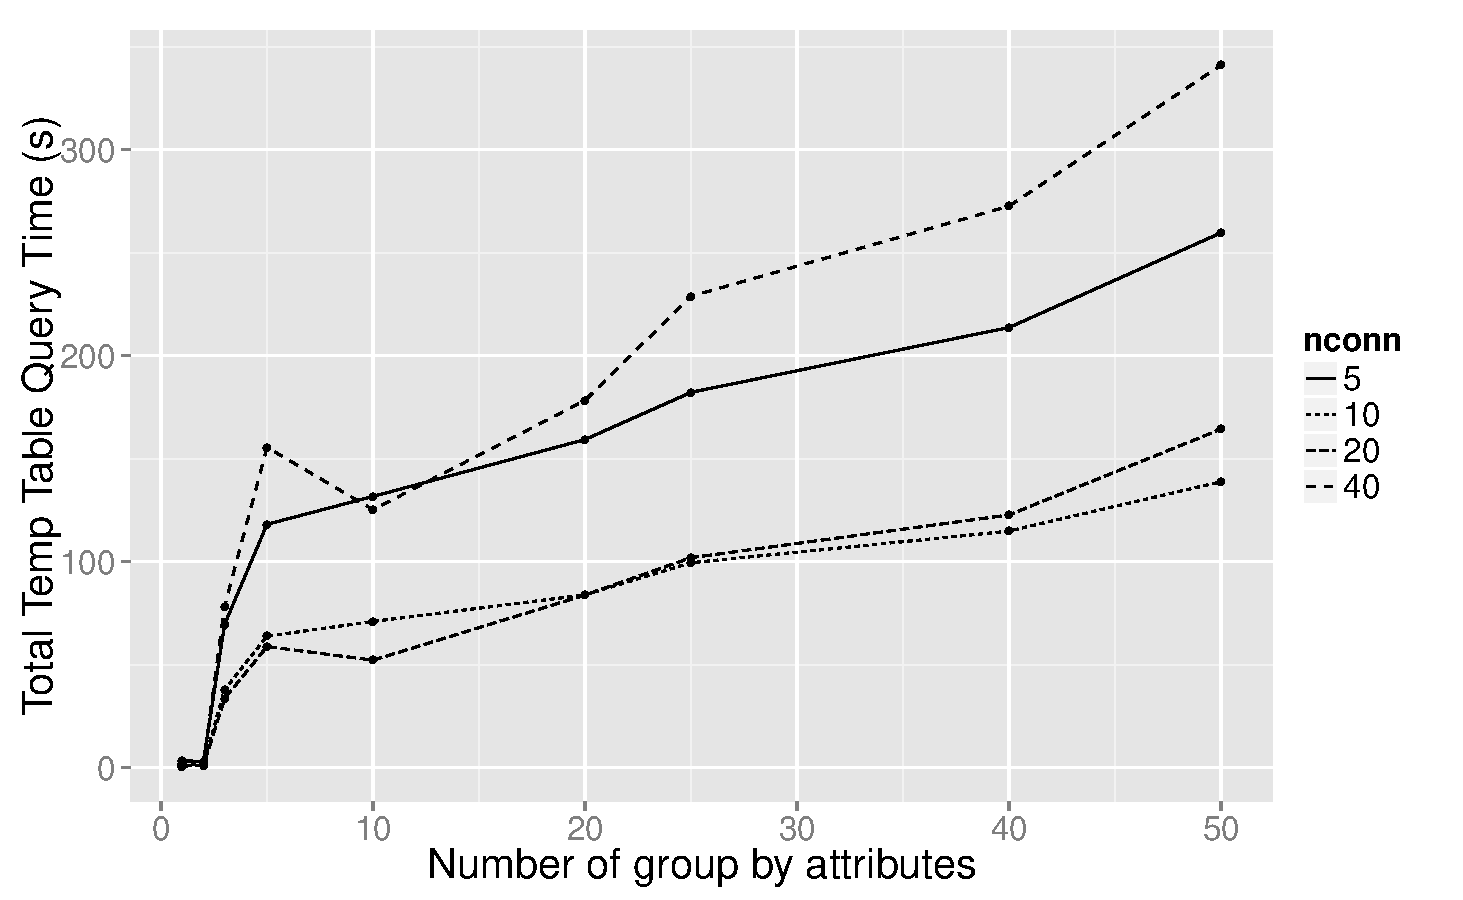
\includegraphics[width=6cm]{Images/mult_gb_tt_query_total.pdf}
     \caption{Total Temp Table Query Time} 
       \label{fig:total_tt_query_time}
\end{figure}

Figure \ref{fig:total_tt_query_time} shows the total time taken to query the
temp tables for all the final views. Note again that the trends in total query
time are not identical to those in average query time because number of query
batches required is inversely proportional to the number of connections.
In Figure \ref{fig:total_tt_query_time}, we see that runs with 5 connections are
slow not because of high average query time but because of the large number of
batches of queries that must be executed. In contrast, runs with 40 connections
require very few batches but have high average query time. 10 - 20 connections
and $n_{GB}=1-2$ achieves the best performance.



{\bf Total Execution Time}: The total execution time for \SeeDB\ is the sum of
time required for the two phases above. Figure \ref{fig:total_time} shows the
total \SeeDB\ execution time for different values of $n_{GB}$ and number of
connections. We observe that the best performance is obtained for
$n_{GB}=2$ and 40 parallel connections.

\begin{figure}[h]
     \centering
    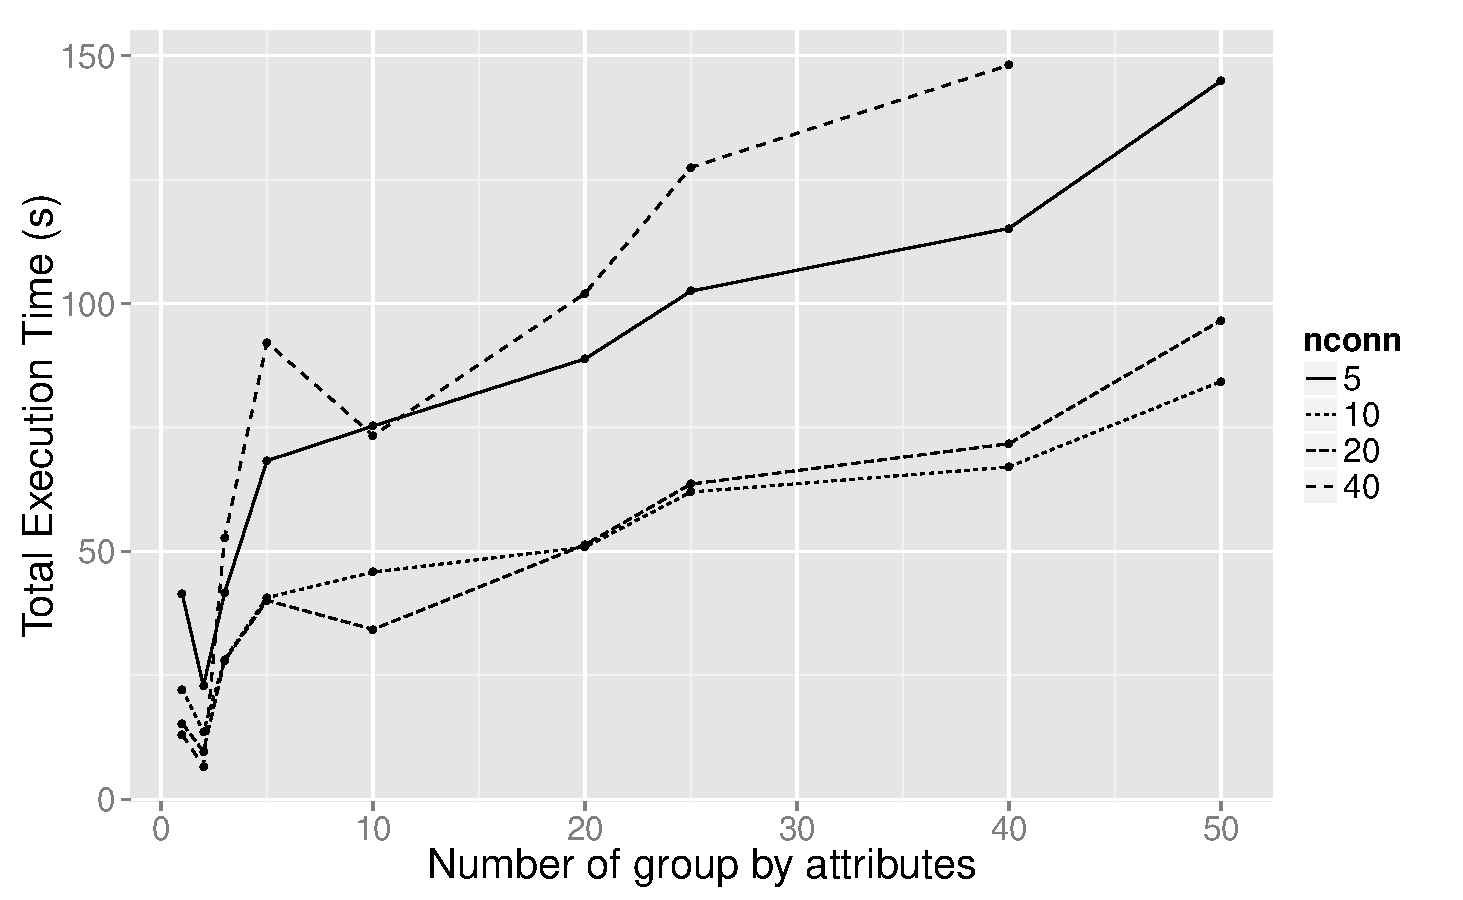
\includegraphics[width=6cm]{Images/mult_gb_total.pdf}
    \caption{Total Execution Time}
  \label{fig:total_time}
\end{figure}

\begin{figure}[h]
  \centering
    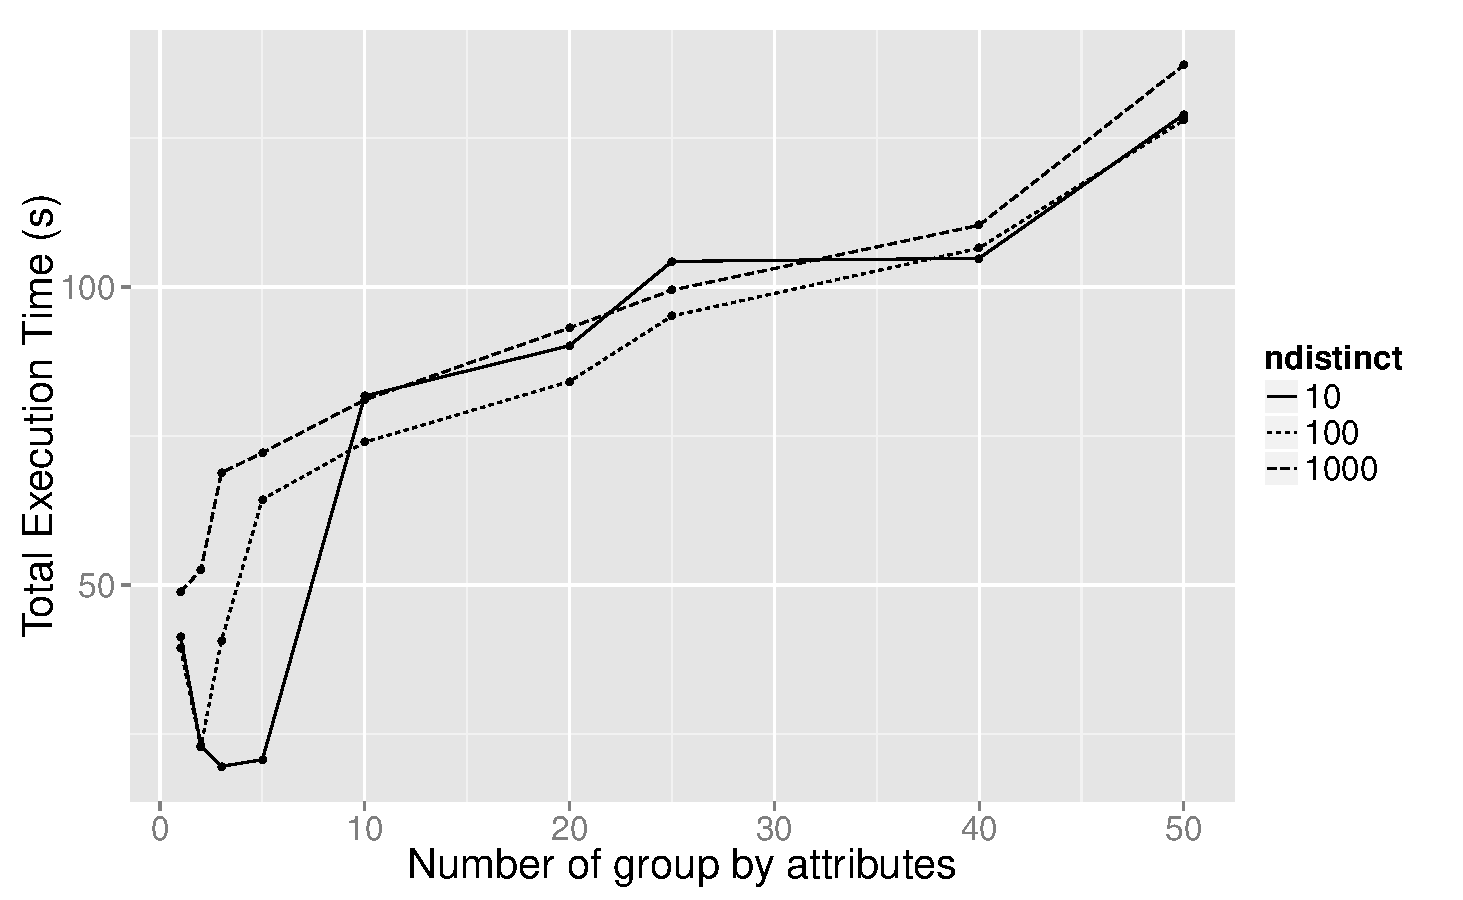
\includegraphics[width=6cm]{Images/mult_gb_diff_distinct.pdf}
    \caption{Total Execution Time vs. Number of Distinct Values} 
  \label{fig:total_time_diff_distinct}

\end{figure}

{\bf Effect of Number of Groups:} The above experiments suggest that $n_{GB}=2$
is the optimal value for the number of group by attributes, both for temp table
creation and querying.
Next we study whether this constraint applies to the number of attributes in the
group by clause or the number of distinct groups produced by the grouping. For
this purpose, we created variants of the Medium dataset (1M rows) where each
dimension attribute had $n$ distinct values with $n$=10\ldots1000. We then
repeated the experiments combining multiple group-bys using these datasets.
Figure \ref{fig:total_time_diff_distinct} shows the results of this test. In the
test dataset, the total number of distinct groups for attributes $a_i$ and $a_j$
is the product of the number of distinct groups for each attribute. We observe
in \ref{fig:total_time_diff_distinct} that the previously-observed minima at
$n_{GB}=2$ is actually a function of the number of distinct groups that are
generated by the multiple-attribute grouping.
Specifically, we observe that the optimal value for the number of distinct
groups is in the range of 10,000 - 100,000. We observe similar trends for temp
table creation and query time.



\subsection{Analytical Model}
\label{sec:model}
In this section, we use insights from the experimental characterization of
various optimizations to develop an analytical model of \SeeDB\ performance.
Table \ref{tab:model_params} defines the various parameters used in our model.

\begin{table}
{\center
\vspace{-10pt}
\begin{tabular}[h]{|c|l|}
\hline
Parameter & Description \\ \hline
$d$ & Number of dimension attributes in table \\
$n$ & Number of rows in input table \\
$n_{tt}$ & Number of rows in temporary table \\
$c_{tt}$ & Number of columns in the temporary table \\
$t_r$ & Time to access a single row of any table \\
$t_c$ & Time to process a single column in a row \\
$t_w$ & Time to write a single row of a table \\
$n_{agg}$ & Number of aggregate attributes computed in a single query \\
$n_{d_{i}}$ & Number of distinct values in attribute $d_i$ \\
$T_{create}$ & Time required to create a temp table \\
$T_{query}$ & Time required to query a temp table \\ 
$b_{create}$ & Number of batches of queries required to create temp tables \\
$b_{query}$ & Number of batches of queries required to query temp tables \\
$n_{conns}$ & Number of queries executing in parallel \\ \hline
\end{tabular}
\vspace{-10pt}
\caption{Analytical model parameters \label{tab:model_params}}
}
\end{table}

% As before, consider the two stages of processing: {\it Temp Table Creation} and
% {\it Temp Table Querying}. In \SeeDB\, these two stages take place in parallel:
% first, we create a set of temp tables; then we query the temp tables and as we
% finish querying existing tables, we create new tables. The creation of new
% tables and querying of old tables happens in parallel. 

As before, we break our model into two parts, {\it Temp Table Creation} or {\it
Phase 1} and {\it Temp Table Querying} or {\it Phase 2}. Note further that in
each of these phases, multiple queries are executing in parallel. We call the
set of queries executing in parallel as a ``batch'' of queries. Suppose that the
total number of queries to be executed is $q$ and $n_{conn}$ queries can be
executed in parallel. Then the total number of batches required to executed all
the queries is $\frac{q}{n_{conn}}$. We denote the number of query batches used
in temp table creation and querying as $b_{create}$ and $b_{query}$ respectively.

We now describe the analytical model for Phase 1 or {\it Temp Table Creation}.
The time required to create a temp table is proportional to the sum of the time
required to query the input table, aggregate measure attributes and finally
write the temp table. We claim that the time taken to process one row of any
table is equal to the constant time to process any record plus the time required
to process all the columns in the record.
\begin{equation*}
T_{create}\ \ =\ \ n \ast \frac{(t_r\ +\ t_c \ast c)}{n_{conn}} \ +\ t_w
\ast n_{tt} \ast (t_r\ +\ t_c \ast c_{tt})
\label{eq:create_time}
\end{equation*}

We can model {\it Temp Table Querying} similarly. Total time to query a temp
table is the time to query a single row of the temp table multiplied by the
number of rows in the table.
\begin{equation*}
T_{query}\ \ =\ \ n_{tt} \ast (t_r\ +\ t_c \ast c_{tt}) 
\label{eq:query_time}
\end{equation*}
A related quantity we model is $b_{query}$, the number of temp table query
batches (Phase 2 batches) that are issued per temp table creation batch (Phase 1 batch).
If $d_{tt}$ is the number of dimension attributes in a temp table and $n_{agg}$
is the number of measure attributes, the given temp table contains results
for ($d_{tt} \ast n_{agg}$) views, and therefore $d_{tt} \ast n_{agg}$ queries
will be made against the table. Further, since each temp table contains $d_{tt}$
dimension attributes, there will be $Min(\frac{d}{d_{tt}}, n_{conn})$ temp
tables being queried in any batch, where $n_{conn}$ is the number of queries executing
in parallel. Therefore, the total number of queries is $d_{tt} \ast n_{agg}$
$\ast$ $Min(\frac{d}{d_{tt}}, n_{conn})$. Finally, since $n_{conn}$ of these queries
can execute at the same time, $b_{query}$ can be modeled as follows:
\begin{equation*}
b_{query}\ \ =\ \ \frac{d_{tt} \ast nAgg \ast Min(\frac{d}{d_{tt}},
n_{conn})}{n_{conn}}
\end{equation*}

Using the three definitions above, we can model the total time taken by \SeeDB\
as shown in Equation \ref{eq:total_time}. If there are $b_{create}$ Phase 1
batches, then the total execution time is equal to the time taken to complete
one batch multiplied by $b_{create}$. In turn, the time taken to complete a
Phase 1 batch is the time taken to create temp tables and subsequently query
them in Phase 2 batches.
Since these two steps take place in parallel, we approximate the completion time
for a Phase 1 batch as the difference between the temp table query time and temp
table creation time.
\begin{equation*}
T_{total}\ \ =\ \|(T_{create} - T_{query} \ast b_{query})\| \ast b_{create}
\label{eq:total_time}
\end{equation*}

We evaluate the accuracy of our model by comparing the model predictions to
actual performance results. Figure \ref{fig:create_time_fitted} shows the
accuracy of our model for predicting time to create temporary tables using
Equation \ref{eq:create_time} (Medium dataset, 1M tuples, 5 connections).
Similarly, Figure \ref{fig:query_time_fitted} shows the accuracy of our model
for predicting time to query temporary tables using Equation
\ref{eq:query_time}. Finally, Figure \ref{fig:total_time_fitted} shows the
accuracy of our model for predicting total execution time as derived in Equation
\ref{eq:total_time}.

\begin{figure}[h]
  \centering
    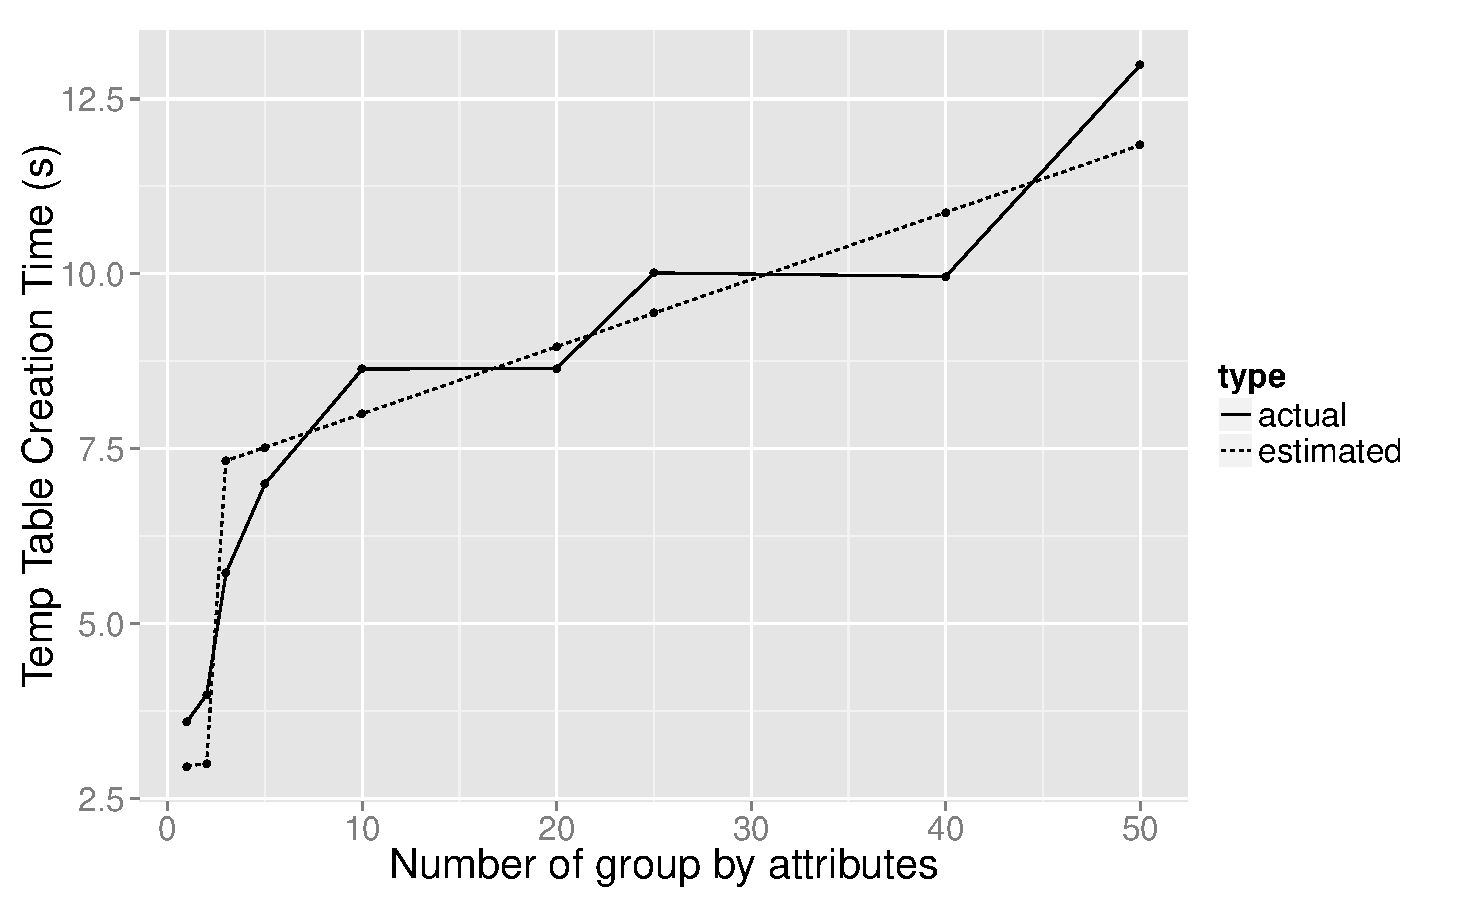
\includegraphics[width=6cm]{Images/create_time_fitted.pdf}
  \caption{Actual and Estimated Temp Table Query Time}
  \label{fig:create_time_fitted}
  
\end{figure}
\begin{figure}[h]
  \centering
    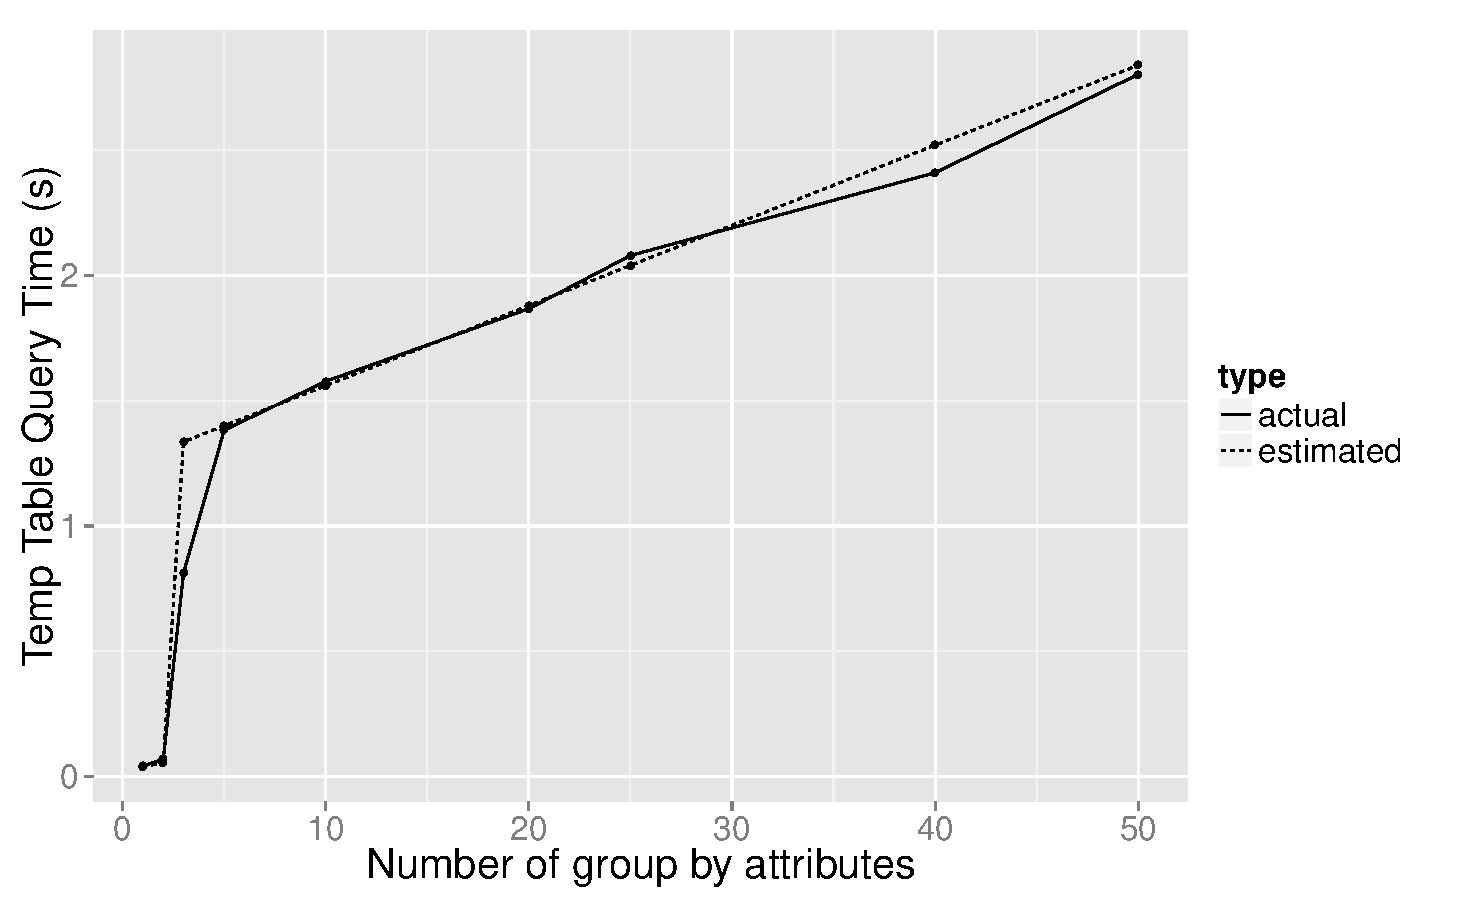
\includegraphics[width=6cm]{Images/query_time_fitted.pdf}
  \caption{Actual and Estimated Temp Table Query Time} 
  \label{fig:query_time_fitted}
\end{figure}

\begin{figure}[h]
  \centering
    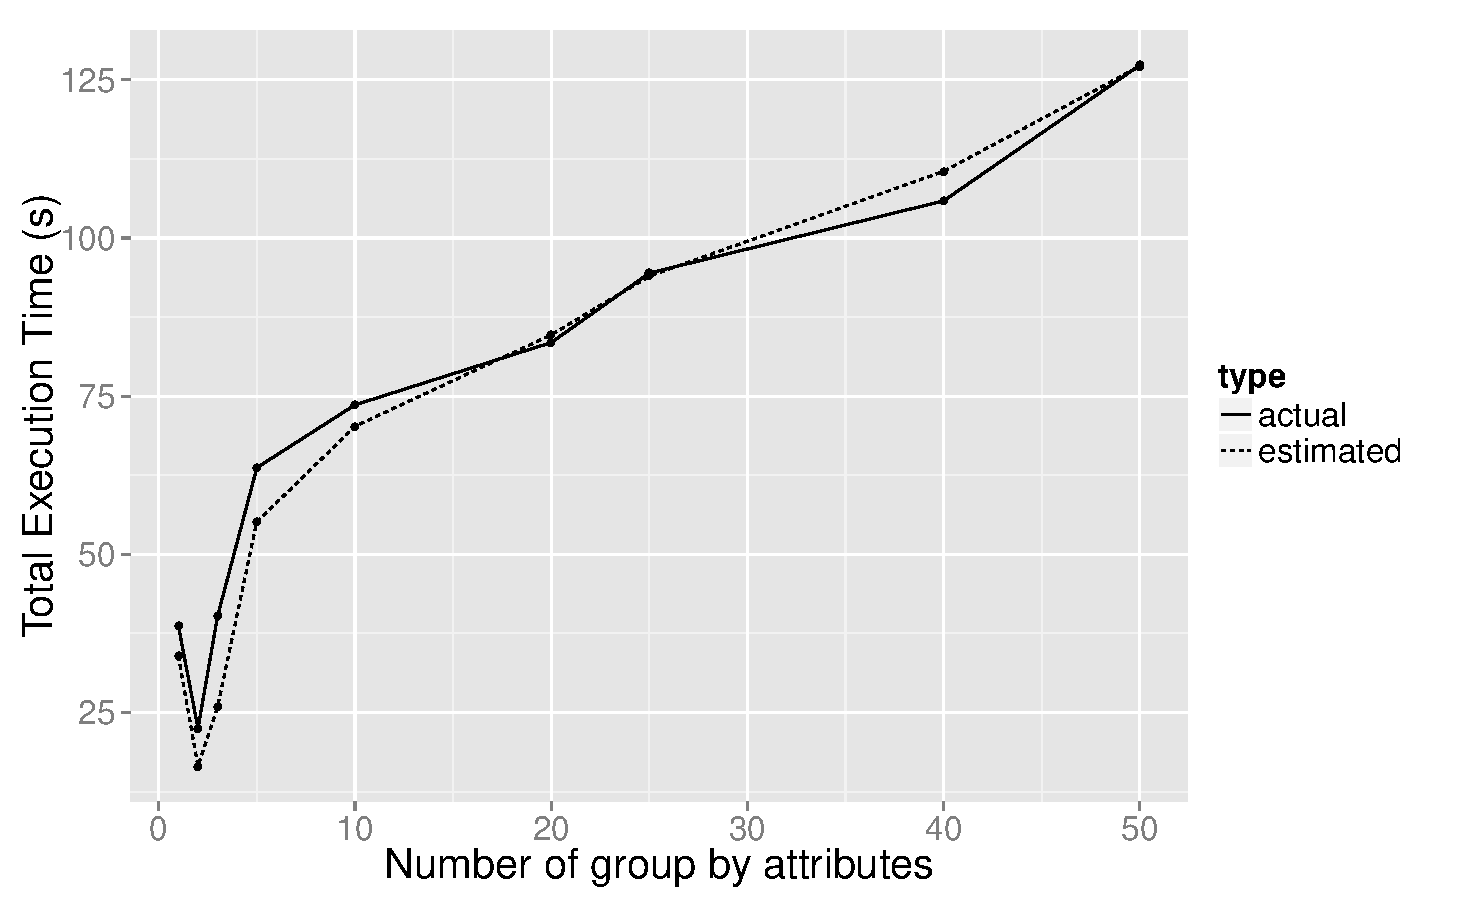
\includegraphics[width=6cm]{Images/total_time_fitted.pdf}
  \caption{Actual and Estimated Total Execution Time} 
    \label{fig:total_time_fitted}
\end{figure}

\subsection{Choosing \SeeDB\ parameters based on the model}

{\bf Choosing Number of Parallel Queries:} The speed up offered by running
queries in parallel depends on the DBMS parameters such as maximum number of
connections, shared buffer size, etc. In our implementation, each phase of
processing can issue up to $n_{conn}$ queries in parallel, so in principle,
there may be up to $2 \ast n_{conn}$ queries running in parallel. Since each
DBMS has a maximum number of queries that can be executed in parallel,
$n_{conn}$ must be set to be smaller than half the maximum number of
connections. The exact number of connections will depend on the other workload
in the system and the size of the dataset. In our setup, $n_{conns}$=40 gives
the best results for a range of dataset sizes and system parameters.

{\bf Choosing $n_{agg}$:} Combining multiple aggregates offers a performance
gain that is almost linear in the number of aggregates, without any significant
penalty. As a result, we set $n_{agg}$ equal to the number of measure attributes
in the table.

{\bf Choosing dimension attributes to combined processing:}  As discussed in
Section \ref{subsec:mult_gb_expt}, the optimal number of distinct groups
consistently falls in the range 10,000 to 100,000. As a result, we set
$n_{groups}$, the maximum number of groups that any query can generate, to
100,000.
This parameter is used to pick dimension attributes that will be combined into a
single view query. For a set of attributes $a_1$\ldots$a_n$, the maximum number
of distinct groups that can be generated is $\prod_i a_i$. This is the worst
case bound since correlation between two attributes can only decrease the number
of distinct groups. \SeeDB\ models the problem of grouping attributes with a
constraint on number of groups as a variant of bin-packing.
Specifically, \SeeDB\ adopts the following problem formulation.

Let $n_{d_{i}}$ be the number of distinct values for dimension attribute $d_i$.
The traditional definition for bin packing states that given bins of size $V$
and $n$ items with size $a_1$\ldots$a_n$, find the minimum integer number of
bins and a corresponding partition of the set of items such that $\sum_{j} a_j$
$\leq$ $V$ for all $a_j$ belong to any given partition. In our setting, there is
a limit on the {\it product} (as opposed to the sum) of the sizes of items. As a
result, we formulate the problem as follows: Given bins (queries) of size $V$
($V$=100,000) and $d$ attributes with sizes $log(n_{d_{i}})$, find
the minimum number of bins and a corresponding partition of the $d$ attributes
such that $\sum_{j} log(n_{d_{j}})$, i.e. $\prod_{j} n_{d_{i}}$, $\leq$ $V$.
Bin-packing has been well studied and we use off-the-shelf software
\cite{glpk} to perform bin-packing on the dimension attributes.

\subsection{Experimental Evaluation with All Optimizations}

We now show performance results for \SeeDB\ using the optimal parameter settings
described above. Specifically, we set $n_{conns}$=40, $n_{agg}$=$m$ (i.e.
number of measure attributes) and $n_{groups}$=100,000 for bin-packing. Further,
we apply the optimization of combinging target and comparison queries for each view. From
Figure \ref{fig:total_speed_up}, we see that the combination of all
optimizations gives us a speedup of about 100X for the Medium and Large
datasets (note the log scale on Y axis). Although the impact of optimizations is
relatively small for the Small dataset, we still observe that the total
execution time is halved. We thus see that the all the optimizations
taken together can enable \SeeDB\ to run at near-interactive response times.

\begin{figure}[h]
  \centering
    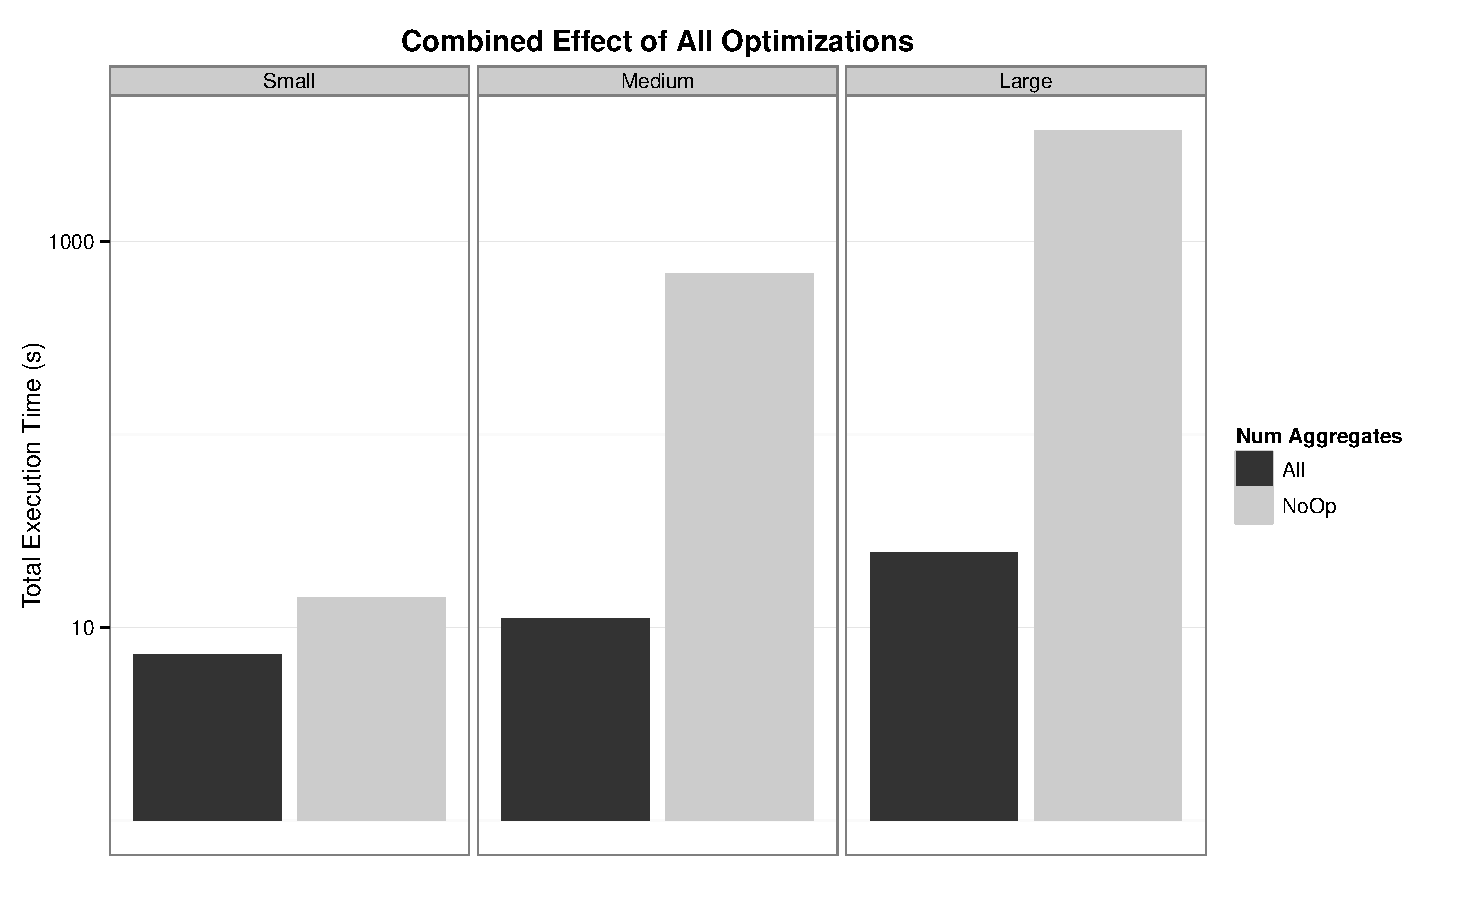
\includegraphics[width=6cm]{Images/total_speedup.pdf}
  \caption{Performance Speedup With Optimizations} 
  \label{fig:total_speed_up}
\end{figure}





\mpv{end-to-end testing with various parameter settings}